% Options for packages loaded elsewhere
\PassOptionsToPackage{unicode}{hyperref}
\PassOptionsToPackage{hyphens}{url}
%
\documentclass[
  ignorenonframetext,
]{beamer}
\usepackage{pgfpages}
\setbeamertemplate{caption}[numbered]
\setbeamertemplate{caption label separator}{: }
\setbeamercolor{caption name}{fg=normal text.fg}
\beamertemplatenavigationsymbolsempty
% Prevent slide breaks in the middle of a paragraph
\widowpenalties 1 10000
\raggedbottom
\setbeamertemplate{part page}{
  \centering
  \begin{beamercolorbox}[sep=16pt,center]{part title}
    \usebeamerfont{part title}\insertpart\par
  \end{beamercolorbox}
}
\setbeamertemplate{section page}{
  \centering
  \begin{beamercolorbox}[sep=12pt,center]{part title}
    \usebeamerfont{section title}\insertsection\par
  \end{beamercolorbox}
}
\setbeamertemplate{subsection page}{
  \centering
  \begin{beamercolorbox}[sep=8pt,center]{part title}
    \usebeamerfont{subsection title}\insertsubsection\par
  \end{beamercolorbox}
}
\AtBeginPart{
  \frame{\partpage}
}
\AtBeginSection{
  \ifbibliography
  \else
    \frame{\sectionpage}
  \fi
}
\AtBeginSubsection{
  \frame{\subsectionpage}
}
\usepackage{amsmath,amssymb}
\usepackage{lmodern}
\usepackage{iftex}
\ifPDFTeX
  \usepackage[T1]{fontenc}
  \usepackage[utf8]{inputenc}
  \usepackage{textcomp} % provide euro and other symbols
\else % if luatex or xetex
  \usepackage{unicode-math}
  \defaultfontfeatures{Scale=MatchLowercase}
  \defaultfontfeatures[\rmfamily]{Ligatures=TeX,Scale=1}
\fi
% Use upquote if available, for straight quotes in verbatim environments
\IfFileExists{upquote.sty}{\usepackage{upquote}}{}
\IfFileExists{microtype.sty}{% use microtype if available
  \usepackage[]{microtype}
  \UseMicrotypeSet[protrusion]{basicmath} % disable protrusion for tt fonts
}{}
\makeatletter
\@ifundefined{KOMAClassName}{% if non-KOMA class
  \IfFileExists{parskip.sty}{%
    \usepackage{parskip}
  }{% else
    \setlength{\parindent}{0pt}
    \setlength{\parskip}{6pt plus 2pt minus 1pt}}
}{% if KOMA class
  \KOMAoptions{parskip=half}}
\makeatother
\usepackage{xcolor}
\newif\ifbibliography
\setlength{\emergencystretch}{3em} % prevent overfull lines
\providecommand{\tightlist}{%
  \setlength{\itemsep}{0pt}\setlength{\parskip}{0pt}}
\setcounter{secnumdepth}{-\maxdimen} % remove section numbering
\usepackage{booktabs}
\usepackage{longtable}
\usepackage{array}
\usepackage{multirow}
\usepackage{wrapfig}
\usepackage{float}
\usepackage{colortbl}
\usepackage{pdflscape}
\usepackage{tabu}
\usepackage{threeparttable}
\usepackage{csquotes}
\usepackage{makecell}
\ifLuaTeX
  \usepackage{selnolig}  % disable illegal ligatures
\fi
\IfFileExists{bookmark.sty}{\usepackage{bookmark}}{\usepackage{hyperref}}
\IfFileExists{xurl.sty}{\usepackage{xurl}}{} % add URL line breaks if available
\urlstyle{same} % disable monospaced font for URLs
\hypersetup{
  pdftitle={Title},
  pdfauthor={Filippo Gambarota},
  hidelinks,
  pdfcreator={LaTeX via pandoc}}

\title{Title}
\subtitle{Subtitle}
\author{Filippo Gambarota}
\date{2022-2023}

\begin{document}
\frame{\titlepage}

\begin{frame}{An example\ldots{}}
\protect\hypertarget{an-example}{}
We measure the \textbf{accuracy} of students to questions of
\textbf{increasing difficulty}, from 0 = easy to 7 = very hard. Thus we
have binary data where 1 = passed and 0 = failed.

\begin{table}
\centering\begingroup\fontsize{7}{9}\selectfont

\begin{tabular}{lll}
\toprule
\textbf{id} & \textbf{difficulty} & \textbf{y}\\
\midrule
1 & 0 & 1\\
2 & 0 & 1\\
3 & 0 & 1\\
4 & 0 & 1\\
... & ... & ...\\
\addlinespace
157 & 7 & 0\\
158 & 7 & 0\\
159 & 7 & 0\\
160 & 7 & 0\\
\bottomrule
\end{tabular}
\endgroup{}
\end{table}
\end{frame}

\begin{frame}{An example\ldots{}}
\protect\hypertarget{an-example-1}{}
\begin{center}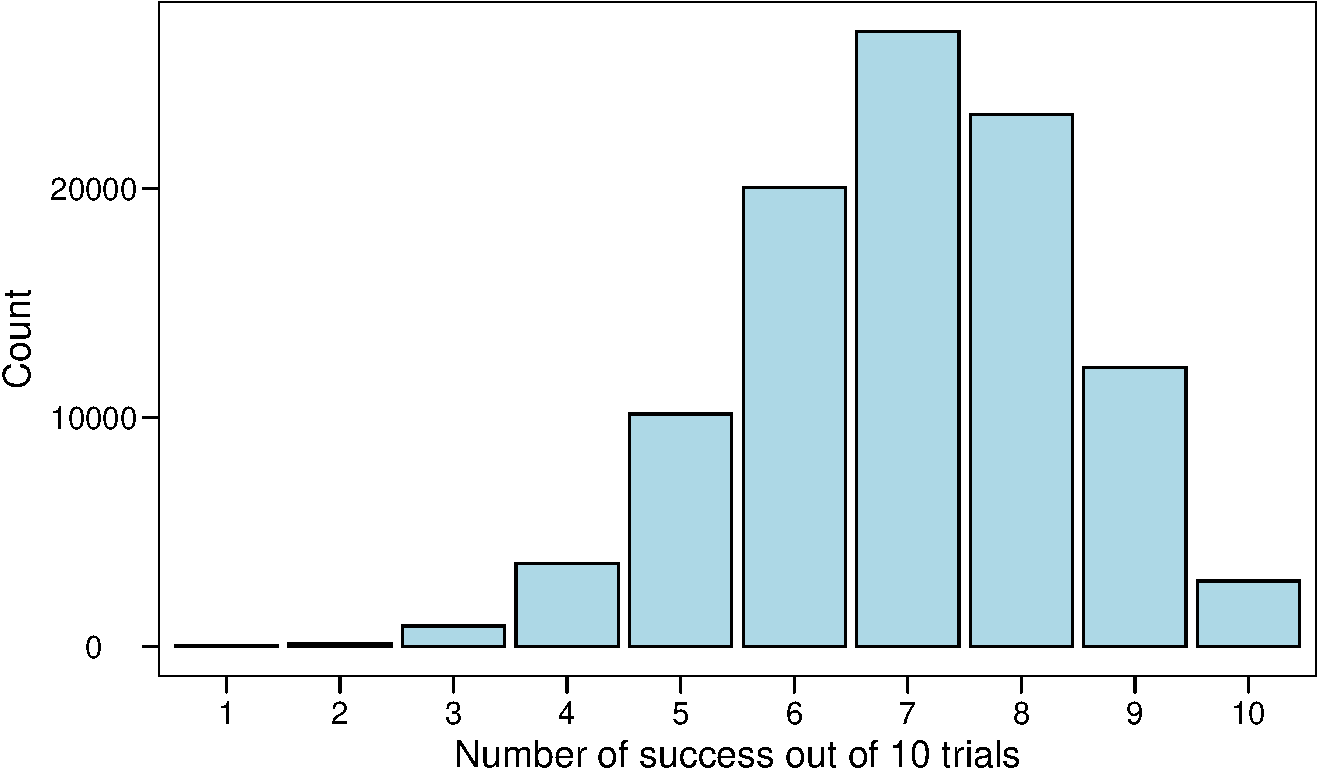
\includegraphics[width=0.8\linewidth]{intro_files/figure-beamer/unnamed-chunk-3-1} \end{center}
\end{frame}

\begin{frame}[fragile]{Fitting a linear model}
\protect\hypertarget{fitting-a-linear-model}{}
Let's try to fit a regression line as
\texttt{y\ \textasciitilde{}\ accuracy}:

\begin{center}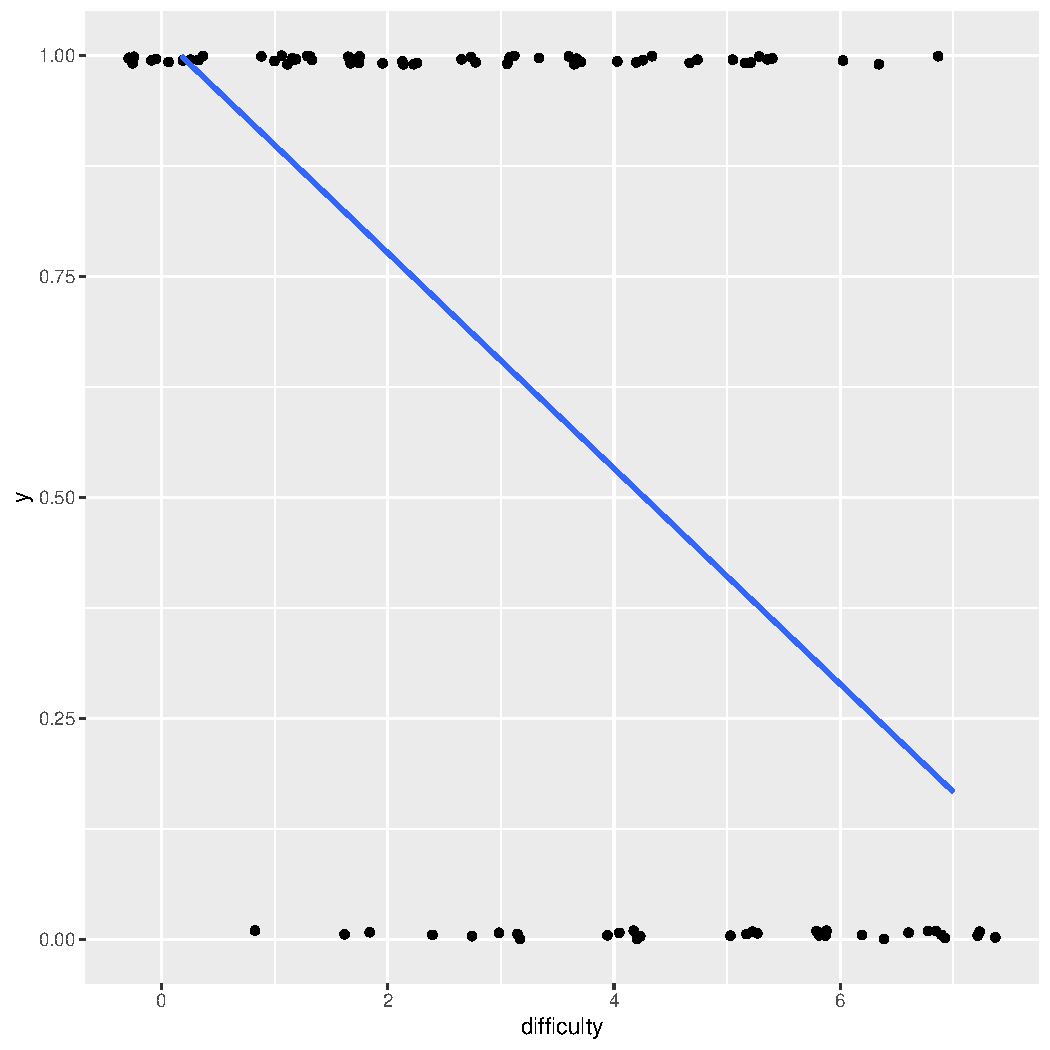
\includegraphics[width=0.8\linewidth]{intro_files/figure-beamer/lm-binary-example-1} \end{center}
\end{frame}

\begin{frame}{Fitting a linear model}
\protect\hypertarget{fitting-a-linear-model-1}{}
\begin{columns}
\begin{column}{0.3\textwidth}


\begin{center}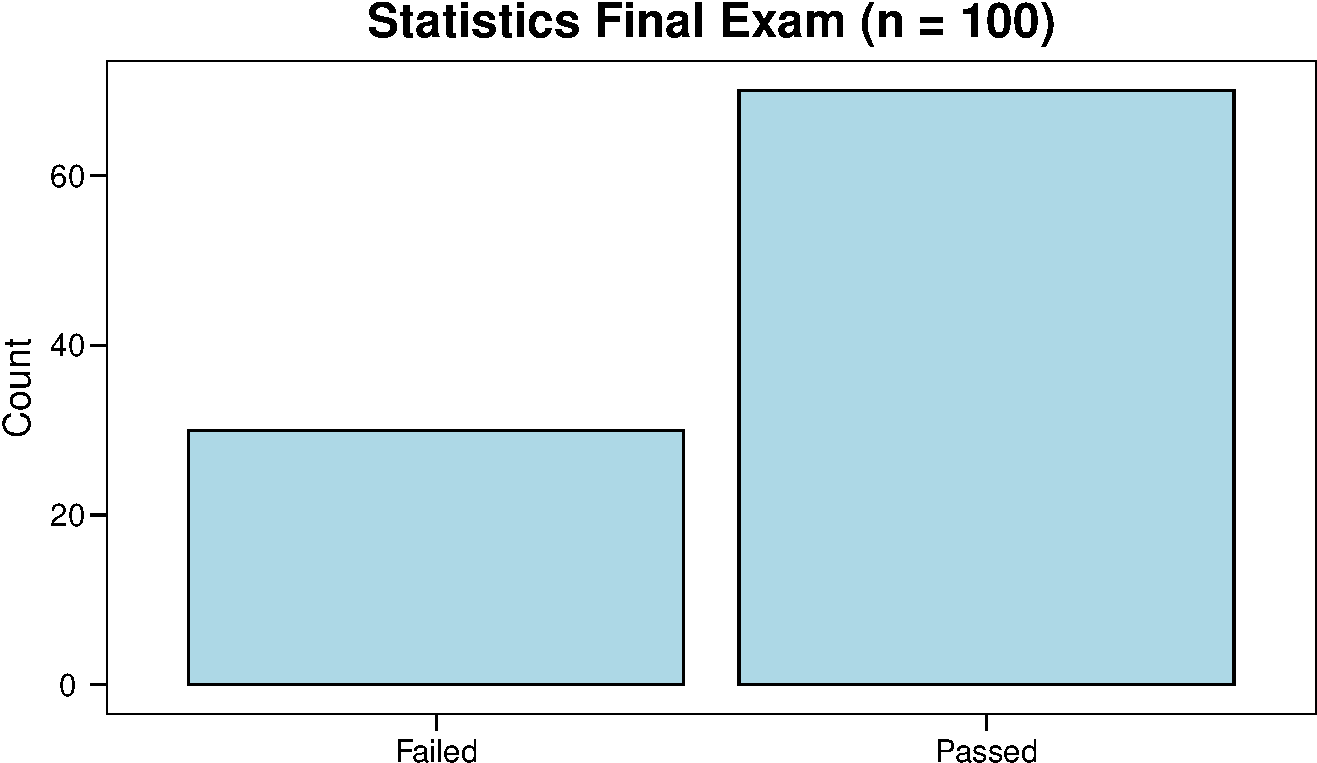
\includegraphics[width=0.8\linewidth]{intro_files/figure-beamer/unnamed-chunk-4-1} \end{center}

\end{column}
\begin{column}{0.7\textwidth}

\begin{itemize}
    \item It is appropriate?
    \item The model is (more or less) capturing the relationship
    \item As the difficulty increases, the accuracy decreases
\end{itemize}

\end{column}
\end{columns}
\end{frame}

\begin{frame}{Fitting a linear model}
\protect\hypertarget{fitting-a-linear-model-2}{}
\begin{displayquote}
"All models are wrong, some are useful."

\hfill --- George Box
\end{displayquote}

\begin{itemize}
\tightlist
\item
  The model is capturing the decreasing relationship! GOOD!
\item
  The model is doing something strange, do you see something strange?
\end{itemize}
\end{frame}

\begin{frame}{Fitting a linear model, problems\ldots{}}
\protect\hypertarget{fitting-a-linear-model-problems}{}
Let's predict some unobserved values:

\begin{center}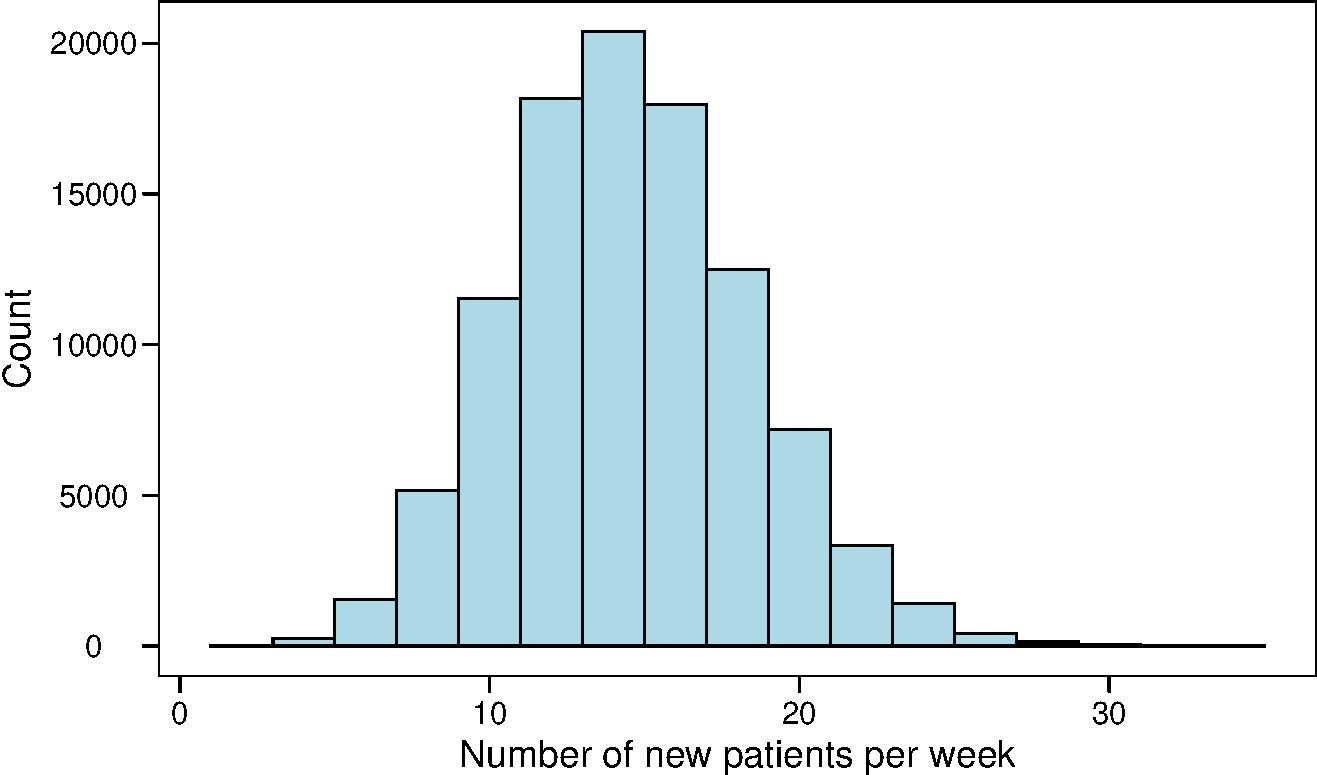
\includegraphics[width=0.8\linewidth]{intro_files/figure-beamer/unnamed-chunk-5-1} \end{center}
\end{frame}

\begin{frame}[fragile]{Fitting a linear model, problems\ldots{}}
\protect\hypertarget{fitting-a-linear-model-problems-1}{}
\begin{itemize}
\tightlist
\item
  Impossible predictions, probabilities are bounded between 0 and 1
\item
  If the \texttt{x} variable has a wider range, the model is completely
  wrong
\item
  Despite somehow \emph{useful}, the model is seriously \emph{flawed}
\end{itemize}

\begin{block}{Block title}
We need a model take take into account our dependent variables. Let's switch to the \textbf{generalized linear models}! 
\end{block}
\end{frame}

\begin{frame}{Not only binary data\ldots{}}
\protect\hypertarget{not-only-binary-data}{}
\begin{center}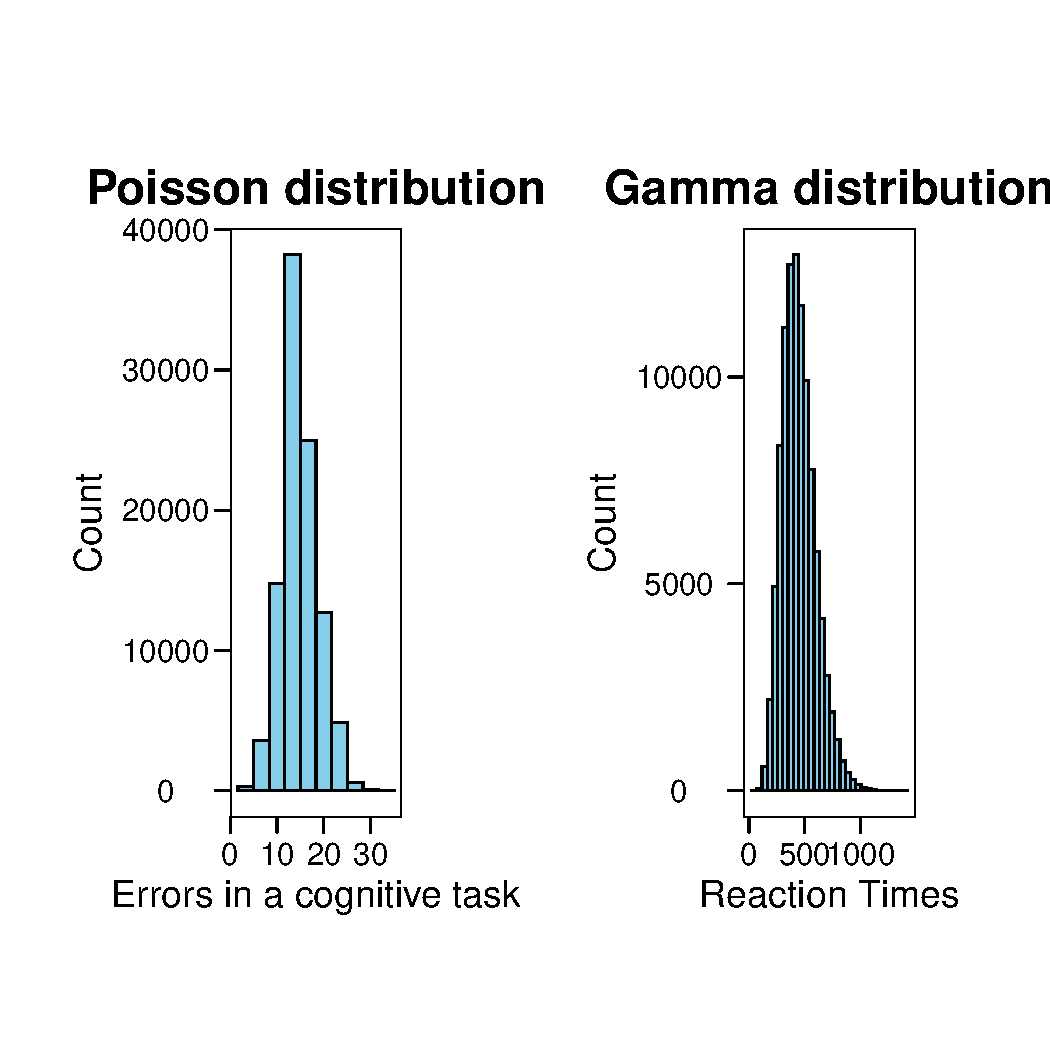
\includegraphics[width=0.8\linewidth]{intro_files/figure-beamer/unnamed-chunk-6-1} \end{center}
\end{frame}

\begin{frame}{Why the linear model is not appropriate?}
\protect\hypertarget{why-the-linear-model-is-not-appropriate}{}
\begin{center}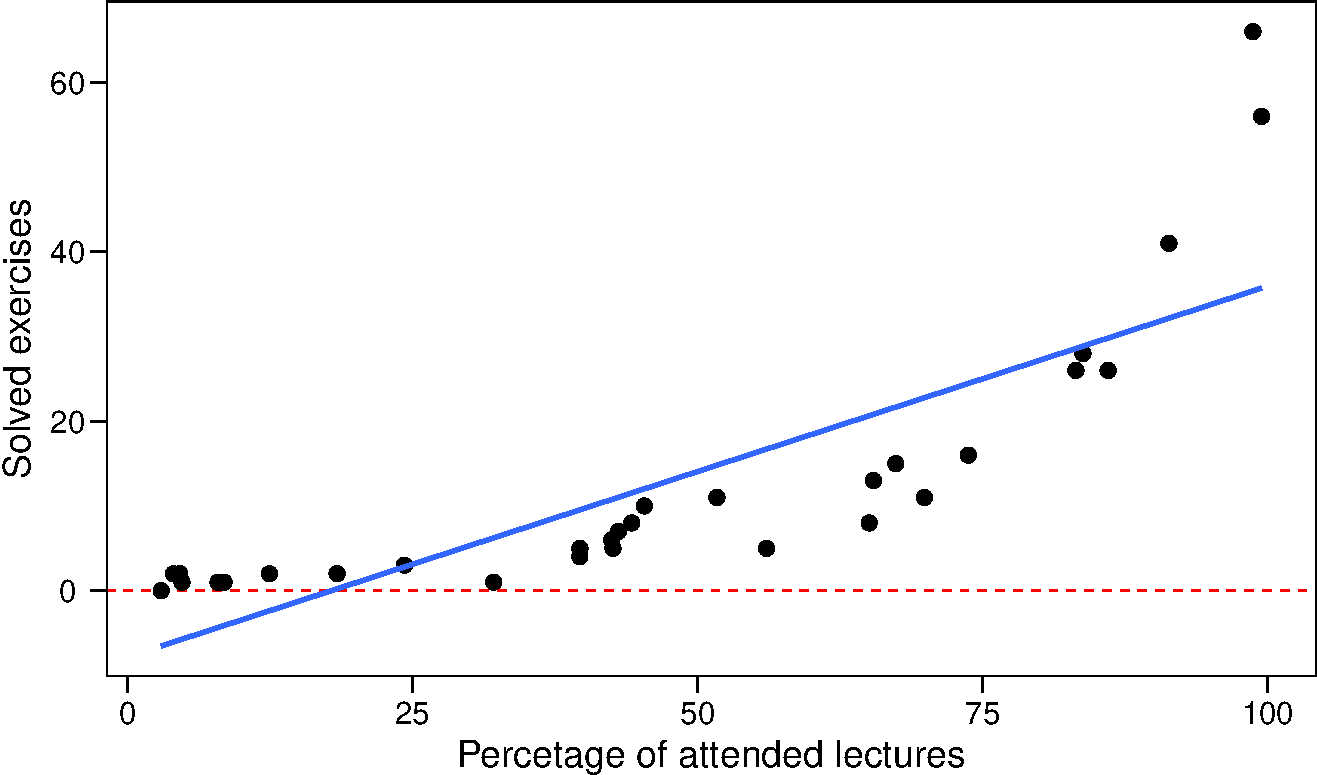
\includegraphics[width=0.8\linewidth]{intro_files/figure-beamer/unnamed-chunk-7-1} \end{center}
\end{frame}

\begin{frame}{Ciao}
\protect\hypertarget{ciao}{}
\begin{center}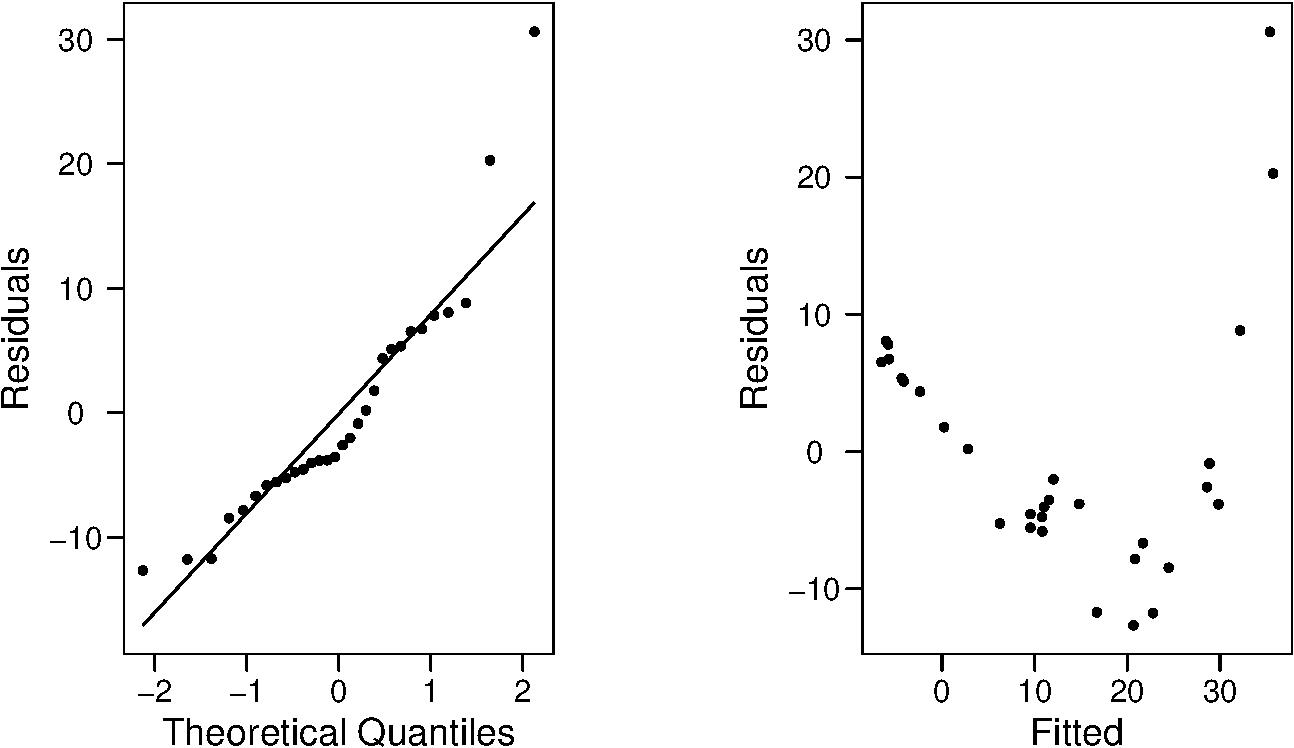
\includegraphics[width=0.8\linewidth]{intro_files/figure-beamer/unnamed-chunk-8-1} \end{center}
\end{frame}

\begin{frame}{Logit and Probability}
\protect\hypertarget{logit-and-probability}{}
\begin{columns}
\begin{column}{0.3\textwidth}

The logit transformation map probabilities with range $(0, 1)$ to $(-\infty, \infty)$.

\begin{multiline}
logit(\pi) = log \left( \frac{\pi}{1 - \pi}\right) \\
logit(\pi)^{-1} = \frac{e^{\pi}}{1 + e^{\pi}}
\end{multiline}

\end{column}
\begin{column}{0.7\textwidth}


\begin{center}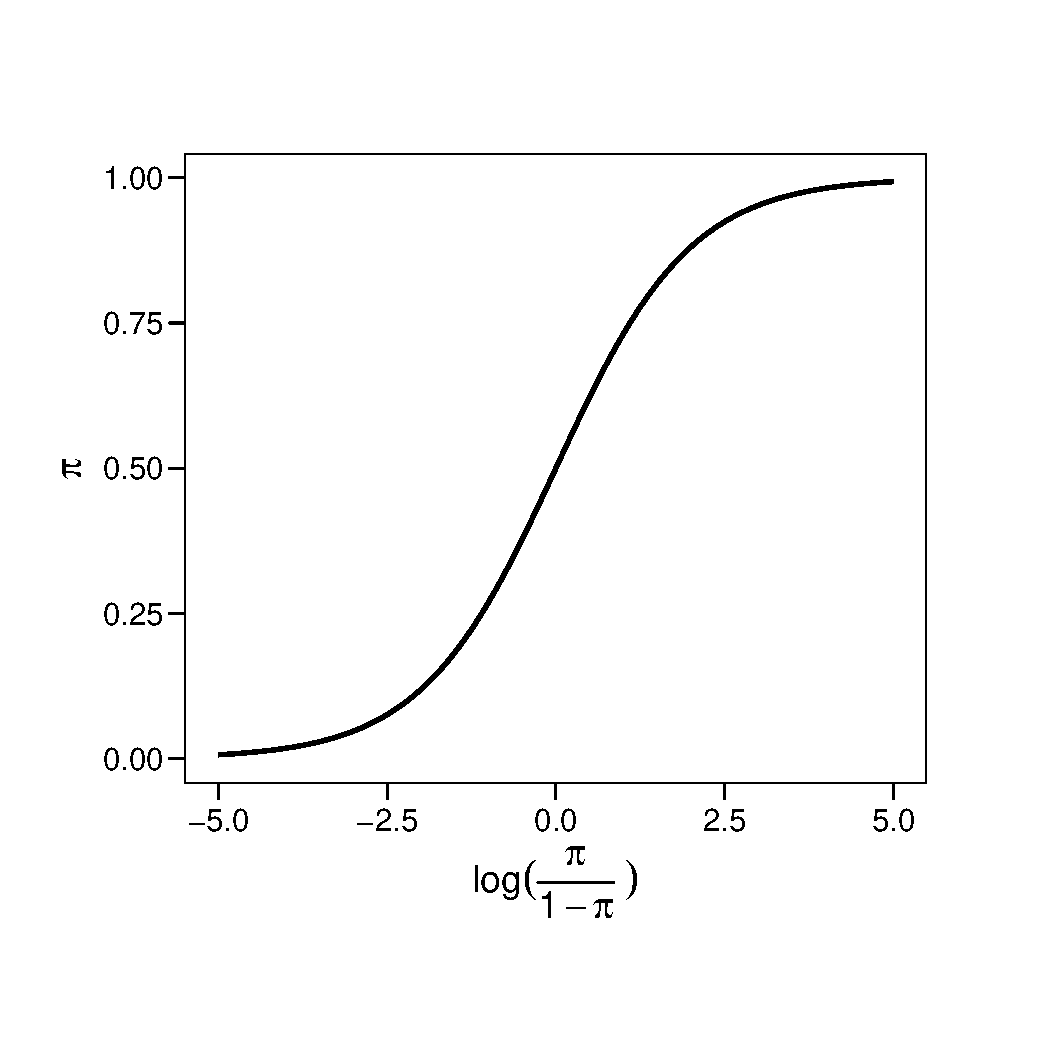
\includegraphics[width=0.8\linewidth]{intro_files/figure-beamer/unnamed-chunk-9-1} \end{center}

\end{column}
\end{columns}
\end{frame}

\begin{frame}{Recipe for a \textbf{G}eneralized \textbf{L}inear
\textbf{M}odel}
\protect\hypertarget{recipe-for-a-generalized-linear-model}{}
\begin{enumerate}
\tightlist
\item
  A vector of outcome data \(y = (y_1,..., y_n)\)
\item
  A matrix of predictors X and vector of coefficients \(\beta\), forming
  a linear predictor vector \(X\beta\)
\item
  A link function \(g\), yielding a vector of transformed data
  \(\hat y = g^{−1}(X\beta)\) that are used to model the data
\end{enumerate}
\end{frame}

\begin{frame}{For example in logistic regression}
\protect\hypertarget{for-example-in-logistic-regression}{}
\begin{itemize}
\tightlist
\item
  The link function \(g\) is the \textbf{logit} function
  \(logit(\pi) = log \left( \frac{\pi}{1-\pi}\right)\) and the inverse
  is \(logit(\pi)^{-1} = \frac{e^{\pi}}{1 + e^{\pi}}\)
\item
  The relationship between \(y\) and \(x\) is linear on the transformed
  space (thus applying \(g\)) but non linear on the original space (thus
  applying \(g^{-1}\)).
\item
  In this way, we can reason as in a standard linear model when we are
  in the transformed space. The drawback is that coming back on the
  original scale the relationship is no longer linear
\end{itemize}
\end{frame}

\begin{frame}{Linear on the \(g(x)\) scale but not on the \(g^{-1}(x)\)
scale}
\protect\hypertarget{linear-on-the-gx-scale-but-not-on-the-g-1x-scale}{}
\begin{center}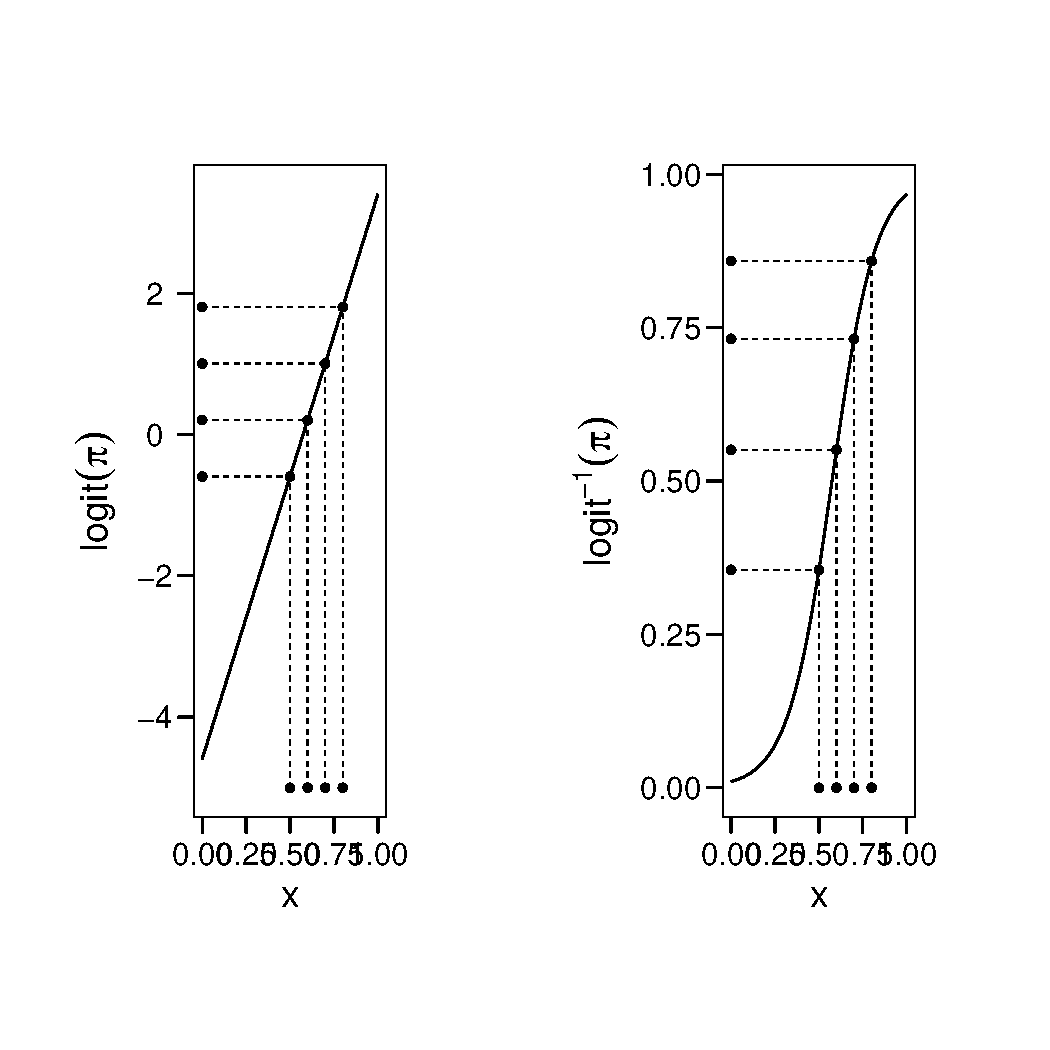
\includegraphics[width=0.8\linewidth]{intro_files/figure-beamer/unnamed-chunk-10-1} \end{center}
\end{frame}

\end{document}
